\section{Experimental validation}
\label{sec:exps}

We evaluated the predictive performances of our models on several real world networks, directed and undirected. Theirs characteristics and properties are summarized in Table \ref{table:corpus} and detailed descriptions are available in the online Koblenz network collection\footnote{http://konect.uni-koblenz.de/networks/}. For both astro-ph and hep-ph datasets, we used the cleaned version available in the  graph-tool framework.
%The aim of these experiments is to illustrate the advantage of the online inference and to evaluate the performances of the models.
This evaluation is based on a missing weight prediction task using the MSE score. 
For all the datasets, we built a test set by extracting randomly 20 percent of the edges of the network and about the same amount of non-linked pairs of nodes. The remaining data constitutes the training set. We repeated this sampling 10 times with different seeds to cross validate our results. The average values (and standard deviations) computed on the ten sub-training sets are reported as final results.

\begin{table*}[t]
\bgroup
\def\arraystretch{1} % 1 is the default, change whatever you need
	
\caption{Datasets networks used to train the models. Type A is for co-authorship, type C is for communication, type H is for hyperlinks, type L is for lexical network and I for interaction network.}

\resizebox{\textwidth}{!}{
\begin{tabular}{lrrrrcrrrr}
%\Xhline{2\arrayrulewidth}
\toprule
 Datasets     &   Nodes &   Edges &   Density & Directed  &    Diameter &   \multicolumn{3}{c}{Weights}  	& type     \\
 \cmidrule(l){7-9}  &   &   	  &   $\times 10^{-3}$		  & 		  &  		   	&  mean & std  & max             \\
%\hline
\midrule
astro-ph      & 16,706  & 121,251   & 0.87  & False & 14 & 1.8  & 3.3  & 306  & A  \\
%cond-mat     & 16,726  & 47,594    & 0.000 & False & 18 & 3.1  & 7.2  & 544  & A  \\
hep-th        & 8,361   & 15,751    & 0.45  & False & 1  & 5.2  & 16   & 1226 & A  \\
%netscience   & 1,589   & 2,742     & 0.002 & False & 2  & 2.2  & 1.9  & 33   & A  \\
moreno\_names & 1,773   & 9,131     & 5.81  & False & 8  & 1.8  & 3.0  & 100  & L  \\
manufacturing & 167     & 5,783     & 208   & True  & 3  & 14.3 & 44.9 & 1458 & C  \\
fb\_uc        & 1,899   & 20,296    & 5.63  & True  & 4  & 2.8  & 4.7  & 98   & C  \\
digg\_reply   & 30,398  & 85,247    & 0.09  & True  & 11 & 2.0  & 0.2  & 26   & C  \\
slashdot      & 51,083  & 130,370   & 0.05  & True  & 11 & 2.1  & 0.3  & 18   & C  \\
enron         & 87,273  & 320,154   & 0.04  & True  & 15 & 3.4  & 12.4 & 3904 & C  \\
wiki-link     & 100,312 & 887,426   & 0.09  & True  & 14 & 1.7  & 3.0  & 185  & H  \\
prosper-loans & 89,269  & 3,330,225 & 0.42  & True  & 2  & 2.0  & 0.2  & 16   & I  \\
%\Xhline{2\arrayrulewidth}
\bottomrule
\end{tabular}
}


\egroup
\label{table:corpus}
\end{table*}

\subsection{Experimental setup}


We compared our models with several implementations of the state of the art. In the stochastic block model family, we considered the microcanonical stochastic block model implementation of \cite{peixoto2018nonparametric} which integrates an efficient MCMC inference method and its weighted extension, referred respectively to as SBM-gt and WSBM-gt. In the exponential family, we chose the SBM and WSBM implementations of \cite{aicher2014learning} which use a generic variational inference with several kernels, referred to as SBM-ai for the Bernoulli kernel, WSBM-ai-n for the Normal kernel and WSBM-ai-p for the Poisson kernel. Lastly, we compared also our models to the Edge Partition Model (EPM) proposed by ~\cite{zhou2015} which is based on a MCMC inference.


For the models belonging to the weighted mixed-membership class, WMMSB and EPM, we used the inferred posterior distribution to estimate the missing weights by:
\[
%p(y_{ij} \geq 1 | \Thetah, \Phih) = \sum_{kk'} \thetah_{ik} \thetah_{jk'} e^{-\phih_{kk'}}
\hat y_{ij} | \Thetah, \Phih = \sum_{kk'} \thetah_{ik} \thetah_{jk'} \phih_{kk'}
\]
Since the SBM models have been designed for solving the link prediction task, we do not have a posterior distribution adapted for weight prediction. Therefore, we used a post estimation of the average weight value in each classes interaction based on the observed data. More formally, given $O_{kk'}$, a set of observable links (and non links) between the inferred latent classes $k$ and $k'$, the prediction of a missing link between the classes $k$ and $k'$ is given by:
\[
\hat y_{ij} | e_i \in \text{class } k, e_j \in \text{class }k' = \sum_{y_{ij} \in O_{kk'}} \frac{y_{ij}}{\# O_{kk'}}
\]

Note that we used the same method for the weighted versions of the Aicher and Peixoto SBM models as we observed no significant difference and even better results using this latter estimation.

%For all the datasets, we built a test set by extracting randomly 20 percent of the edges of the network and about the same amount of non-links. The remaining data constitutes the training set. We repetead this sampling 10  times with different seeds to cross validate our results. The average values (and standard deviations) computed on the ten sub-training sets are reported, for each proportion, as final results.

% stopping citerion
For deciding when to stop the inference process, 10\% of the training set serves as a validation set on which the log-likelihood is computed after each minibatch iteration. When the increase of the log-likelihood, averaged over the last 20 measures, is less than 0.001, the inference is stopped. The log-likelihood of a given set of observations $\D_{set}$  is given by:
\begin{equation*}
\log p(\D_{set}) = \sum_{i,j \in \D_{set}} \log p(y_{ij} | \phih_{kk'}) p(k|\thetah_i) p(k'|\thetah_j)
%\log p(\D_{test}) = \sum_{i,j \in \D_{test}} \log p(y_{ij} | \phih_{kk'}) p(k|\thetah_i) p(k'|\thetah_j)
\end{equation*}

For all our models, the gradient step parameters  $\tau$ and $\kappa$ were fixed respectively to  $1024$ and $0.5$, the burn-in period $T_{burnin}$ to $150$; for stratified sampling, $M$ was set to $50$, the size of $s_0^{i,m}, \, 1 \le m \le M$ being equal to the number of nodes to which $i$ is not connected to divided by $M$. For MMSB, the hyperparameters $\lambda_0$ and $\lambda_1$ were set to $0.1$. For WMMSB, the shape and scale parameters $r$ et $p$ were fixed to $1$ and for WMMSB, the beta-gamma hyperparameters were fixed to  $c_0=10$, $r_0=1$, $c=100$ and $\epsilon=10^{-6}$. The number of latent classes $K$ was fixed to $10$ for all models and the latent-class hyperparameters $\alpha_k$ to $\frac{1}{K}$. Our implementation is available online\footnote{https://github.com/***/*** (anonymized)}. 


\begin{table*}[t]
\centering
	\caption{Comparison of models in terms of MSE on different networks for $K=10$.}

\resizebox{\textwidth}{!}{
\begin{tabular}{lllllllll}
\hline
               & MMSB-scvb          & WMMSB-bg                    & EPM                        & SBM-ai             & WSBM-ai-n          & WSBM-ai-p          & SBM-gt             & WSBM-gt              \\                              
\hline                                                                                                                                                                             
 astro-ph      & 36.94 $\pm$ 1.38   & \textbf{25.04} $\pm$ 2.73   & 36.93 $\pm$ 1.43           & 36.85 $\pm$ 1.24   & 36.65 $\pm$ 1.39   & 36.29 $\pm$ 1.82   & 38.22 $\pm$ 1.62   & 36.94 $\pm$ 1.83     \\
 enron         & 119.53 $\pm$ 9.8   & \textbf{103.85} $\pm$ 7.09  & 122.73 $\pm$ 8.86          & 127.13 $\pm$ 7.87  & 130.65 $\pm$ 13.83 & 133.51 $\pm$ 12.11 & 115.25 $\pm$ 8.37  & 126.18 $\pm$ 11.12   \\
 fb\_uc        & 32.92 $\pm$ 2.48   & \textbf{23.85} $\pm$ 2.37   & 25.82  $\pm$ 2.17          & 31.80 $\pm$ 2.95   & 35.95 $\pm$ 3.02   & 34.50 $\pm$ 2.84   & 30.85 $\pm$ 4.31   & 30.76 $\pm$ 4.44     \\
 hep-th        & 235.92 $\pm$ 18.53 & \textbf{148.03} $\pm$ 14.22 & 242.28 $\pm$ 16.9          & 246.93 $\pm$ 27.22 & 242.53 $\pm$ 13.98 & 235.99 $\pm$ 24.01 & 237.81 $\pm$ 21.56 & 224.07 $\pm$ 30.74   \\
 wiki-link     & 12.08 $\pm$ 0.49   & \textbf{9.48} $\pm$ 0.32    & 11.26  $\pm$ 0.15          & 11.86 $\pm$ 0.17   & 11.82 $\pm$ 0.48   & 12.01 $\pm$ 0.25   & 11.99 $\pm$ 0.19   & 11.68 $\pm$ 0.56     \\
 moreno\_names & 12.30 $\pm$ 2.01   & 7.93 $\pm$ 1.58             & \textbf{6.16} $\pm$ 0.99   & 12.92 $\pm$ 3.29   & 13.32 $\pm$ 2.97   & 10.59 $\pm$ 1.97   & 10.00 $\pm$ 2.62   & 9.53 $\pm$ 2.71      \\
 digg-reply    & 4.06 $\pm$ 0.01    & \textbf{0.48} $\pm$ 0.07    & 4.03   $\pm$ 0.02          & 4.06 $\pm$ 0.02    & 4.05 $\pm$ 0.01    & 4.05 $\pm$ 0.01    & 4.04 $\pm$ 0.03    & 4.05 $\pm$ 0.02      \\
 prosper-loans & 4.09 $\pm$ 0.01    & \textbf{0.33} $\pm$ 0.36    & 3.88   $\pm$ 0.01          & 4.08 $\pm$ 0.0     & 4.09 $\pm$ 0.0     & 4.08 $\pm$ 0.0     & 3.95 $\pm$ 0.01    & 3.95 $\pm$ 0.01      \\
 slashdot      & 4.33 $\pm$ 0.01    & \textbf{0.73} $\pm$ 0.08    & 4.24   $\pm$ 0.01          & 4.32 $\pm$ 0.01    & 4.33 $\pm$ 0.01    & 4.35 $\pm$ 0.02    & 4.27 $\pm$ 0.01    & 4.28 $\pm$ 0.01      \\
\hline
\end{tabular}
}


\label{table:mse}
\end{table*}

\subsection{Results}


%%%%%%%%%%%%%%%%%%%%%%%%%%%%%%%%%%%%%%%%%%%%%%%%%%%%%%%%
%%%% Prediction performance
%%%%%%%%%%%%%%%%%%%%%%%%%%%%%%%%%%%%%%%%%%%%%%%%%%%%%%%%

Table \ref{table:mse}, gives the MSE scores for the different models and for all networks. To evaluate the ability of the models to reconstruct the missing weights, we compute the MSE only on the missing edges of the test data. Although the models are also able to predict the presence or absence of edges,  we considered that the question of recovering the edges structure should be addressed separately by a link prediction method. 
As one can note, WMMSB-bg outperforms all the other models on the different datasets except for the network moreno\_names. 
The fact that this network is the only one in the category of linguistic network and that it is relatively small could explain this result. \textbf{CL : je ne suis pas d'accord avec phrase suivante} EPM outperforms other models, apart from WMMSB-bg. The other models expose comparable results.

%%%%%%%%%%%%%%%%%%%%%%%%%%%%%%%%%%%%%%%%%%%%%%%%%%%%%%%%
%%%% Sensibility on K 
%%%%%%%%%%%%%%%%%%%%%%%%%%%%%%%%%%%%%%%%%%%%%%%%%%%%%%%%
 

\begin{figure}[h]
\centering
	
\begin{subfigure}
     \centering
         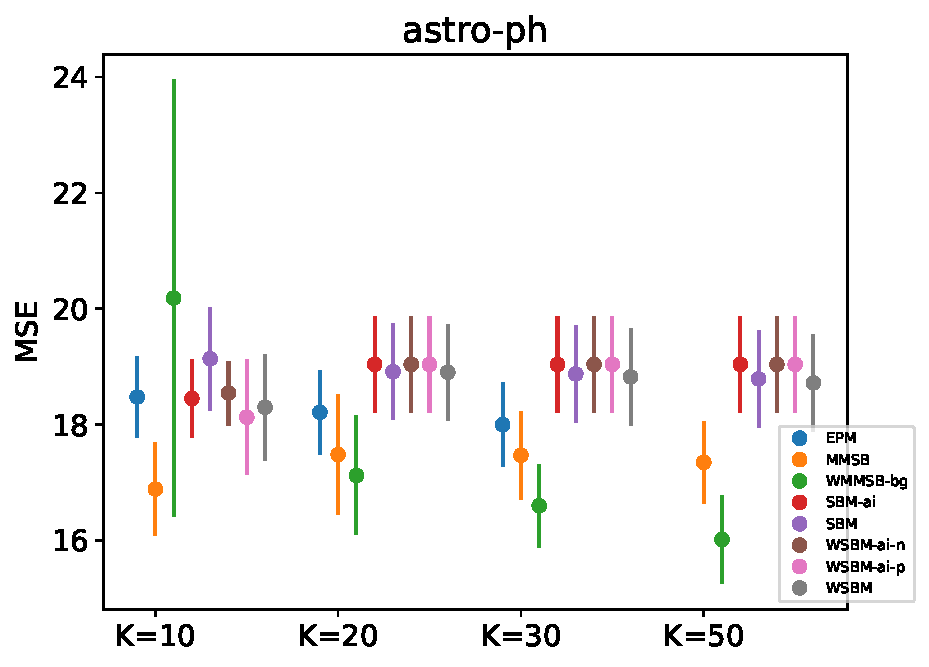
\includegraphics[width=0.23\textwidth]{fig2/astro-ph_wsim3_evo2__}
\end{subfigure}
\begin{subfigure}
         \centering
      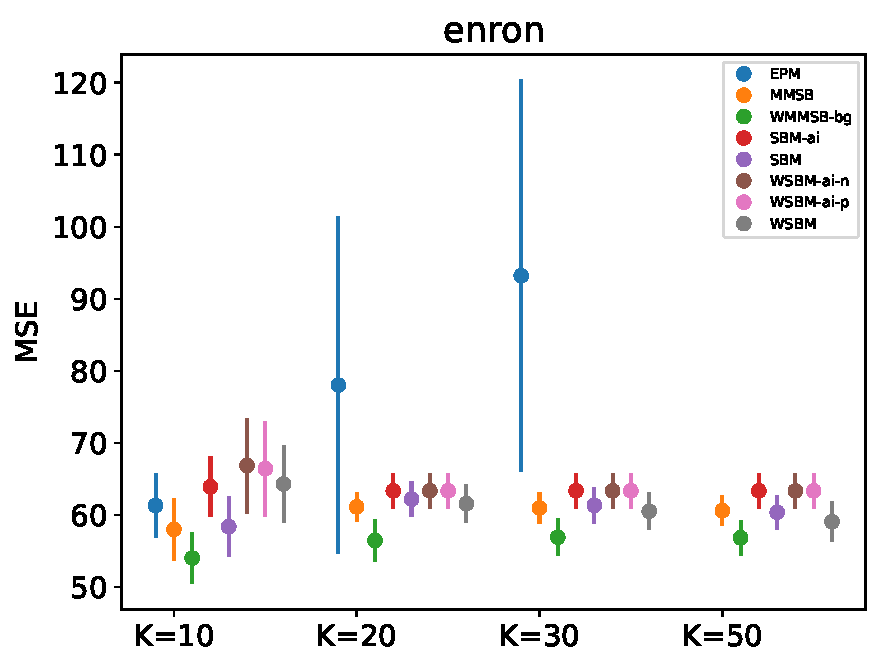
\includegraphics[width=0.23\textwidth]{fig2/enron_wsim3_evo2__}   
\end{subfigure}  
\begin{subfigure}
         \centering          
      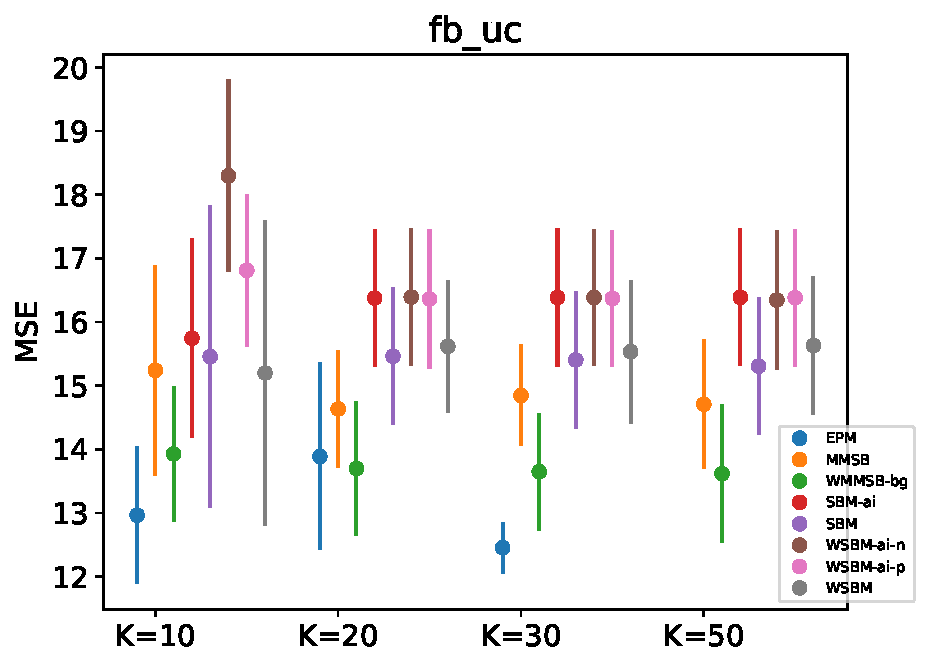
\includegraphics[width=0.23\textwidth]{fig2/fb_uc_wsim3_evo2__}
\end{subfigure}  
\begin{subfigure}
         \centering          
      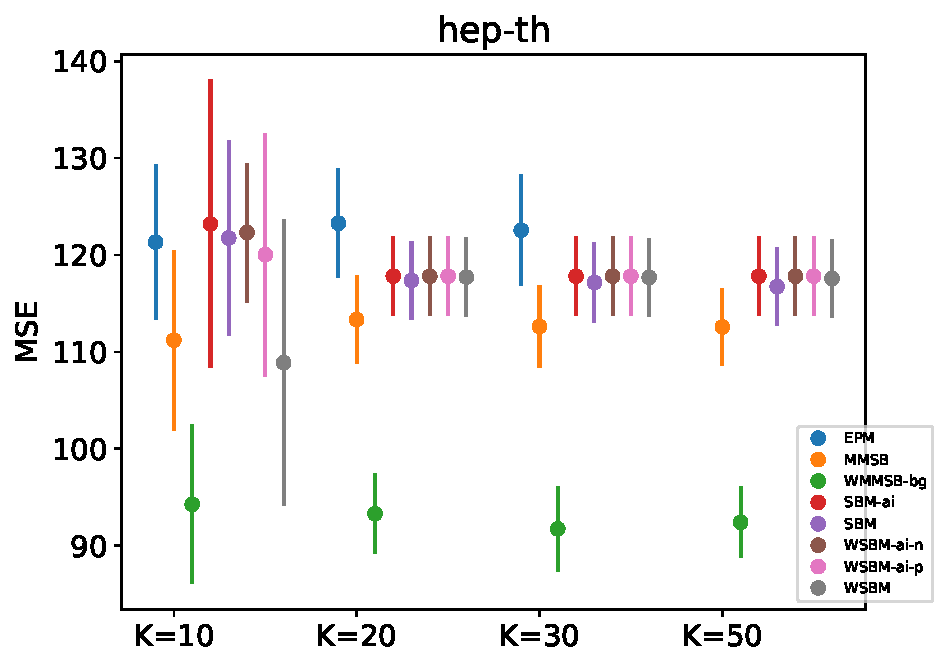
\includegraphics[width=0.23\textwidth]{fig2/hep-th_wsim3_evo2__}
\end{subfigure}  
\begin{subfigure}
         \centering
      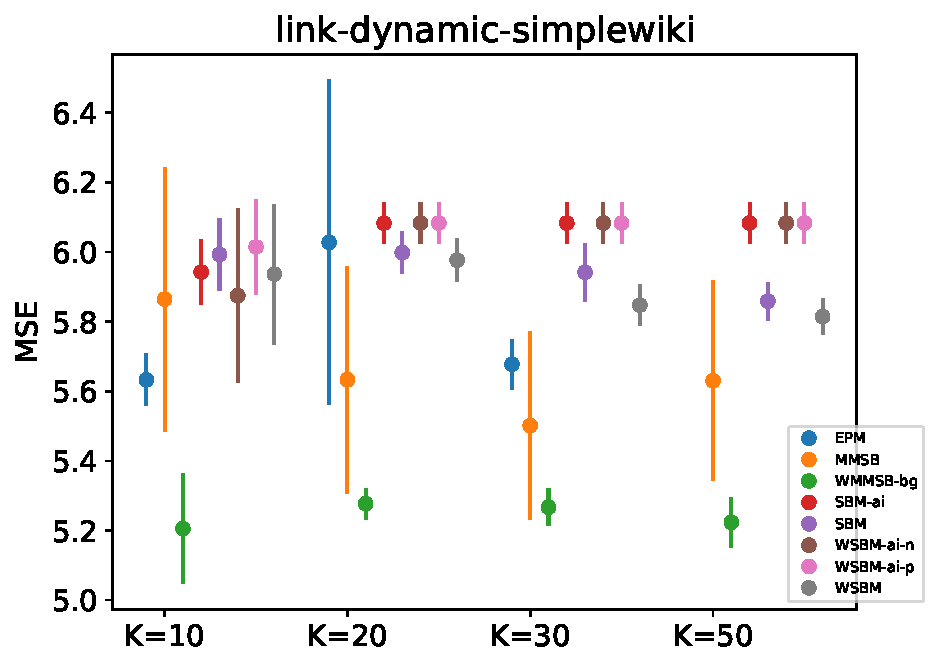
\includegraphics[width=0.23\textwidth]{fig2/wiki-link_wsim3_evo2__}
\end{subfigure} 
\begin{subfigure}
         \centering
      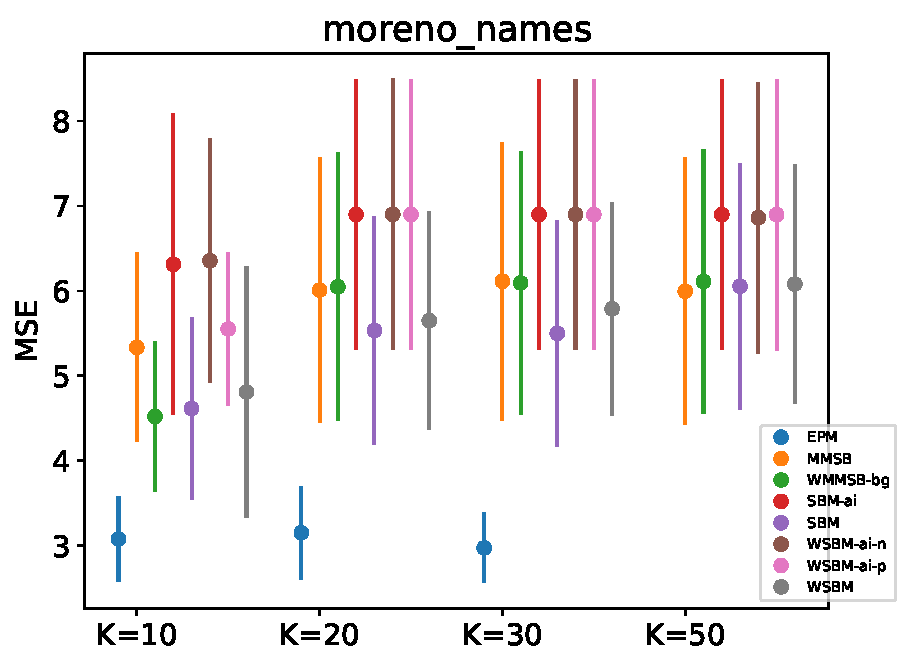
\includegraphics[width=0.23\textwidth]{fig2/moreno_names_wsim3_evo2__}
\end{subfigure} 
\begin{subfigure}
         \centering
      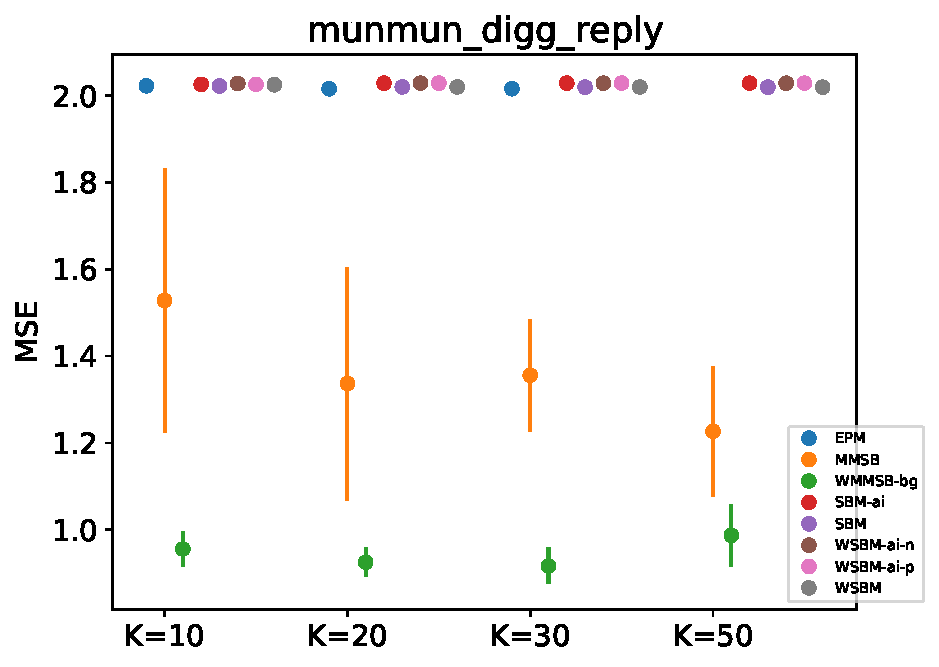
\includegraphics[width=0.23\textwidth]{fig2/digg-reply_wsim3_evo2__}
\end{subfigure} 
\begin{subfigure}
         \centering
      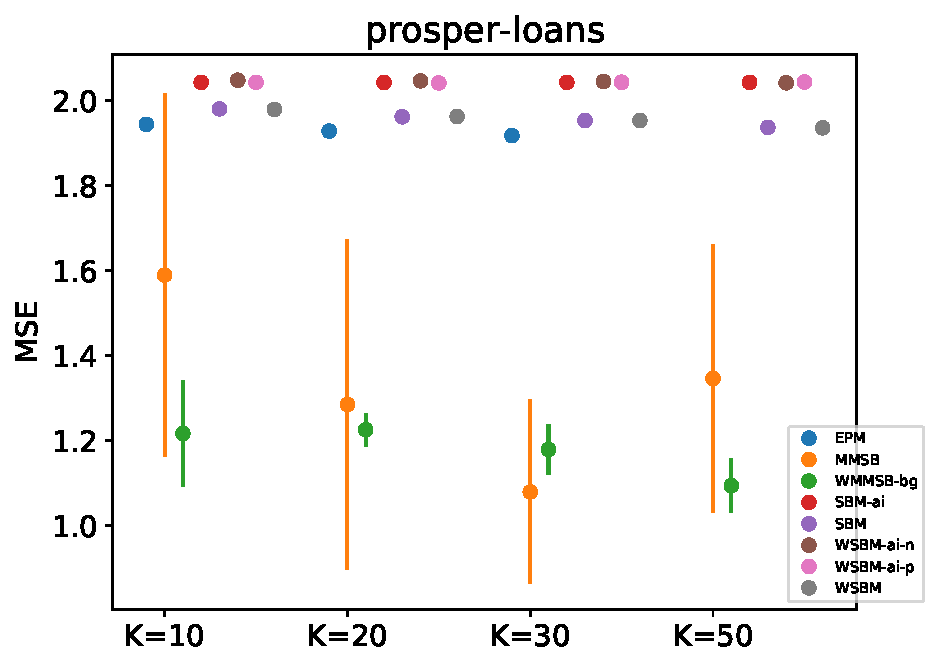
\includegraphics[width=0.23\textwidth]{fig2/prosper-loans_wsim3_evo2__}
\end{subfigure} 
\begin{subfigure}
         \centering
      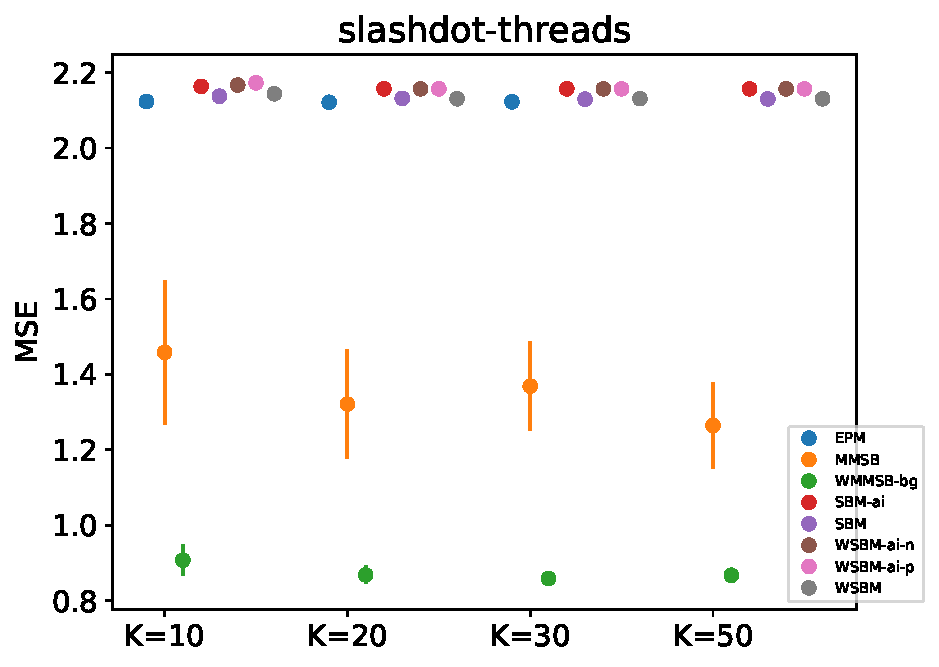
\includegraphics[width=0.23\textwidth]{fig2/slashdot_wsim3_evo2__}
\end{subfigure} 
\caption{Performance sensibility when the number of latent classes vary from $K=10$ to $K=50$.}


   \label{fig:k_evolv}
\end{figure}
Figure \ref{fig:k_evolv} shows the MSE score for $K$, the number of latent classes, varying from 10 to 50 and for six datasets. One can see that for the different methods, the result is relatively stable, in a lesser extent on the networks hep\_th and fb\_uc. Thus, the choice of this parameter has a limited impact on the performances of the models. Nevertheless, it should be notice that for $K$ equals  to 50, EPM has not been able to handle the datasets.

\textbf{CL: Pbl axe 2 indique Wsim et non MSE}

%%%%%%%%%%%%%%%%%%%%%%%%%%%%%%%%%%%%%%%%%%%%%%%%%%%%%%%%
%%%% Timing performance
%%%%%%%%%%%%%%%%%%%%%%%%%%%%%%%%%%%%%%%%%%%%%%%%%%%%%%%%
\begin{table*}[t]
\centering
	\caption{Comparison of models in terms of inference time, in hour, on different datasets for $K=10$. Results are averaged over 10 runs $\pm$ standard deviation. }

\vspace{0.2cm}

\resizebox{\textwidth}{!}{
\begin{tabular}{lllllllll}
\hline
              & MMSB          & WMMSB-bg           & EPM                          & SBM-ai               & WSBM-ai-n        & WSBM-ai-p          & SBM                  & WSBM                  \\
\hline                                                                                                                                                                  
astro-ph      & 0.09 $\pm$ 0.02    & 0.07 $\pm$ 0.02    & \textit{1.08}  $\pm$ 0.01    & 0.08 $\pm$ 0.01      & 0.07 $\pm$ 0.01  & 0.08 $\pm$ 0.02    & \textbf{0.01} $\pm$ 0.01     & 0.03 $\pm$ 0.01          \\
hep-th        & 0.05 $\pm$ 0.01    & 0.08 $\pm$ 0.04    & \textit{0.26}  $\pm$ 0.01    & 0.02 $\pm$ 0.01      & 0.02 $\pm$ 0.01  & 0.02 $\pm$ 0.01    & \textbf{0.01} $\pm$ 0.01     & 0.01 $\pm$ 0.01          \\
moreno\_names & 0.02 $\pm$ 0.02    & 0.01 $\pm$ 0.01    & \textit{0.02}  $\pm$ 0.01    & 0.01 $\pm$ 0.01      & 0.01 $\pm$ 0.01  & 0.01 $\pm$ 0.01    & \textbf{0.01} $\pm$ 0.01     & 0.01 $\pm$ 0.01         \\
fb\_uc        & 0.01 $\pm$ 0.01    & 0.02 $\pm$ 0.01    & \textit{0.02}  $\pm$ 0.01    & 0.01 $\pm$ 0.01      & 0.01 $\pm$ 0.01  & 0.01 $\pm$ 0.01    & \textbf{0.01} $\pm$ 0.01     & 0.01 $\pm$ 0.01           \\
digg-reply    & 0.51 $\pm$ 0.30    & 0.71 $\pm$ 0.27    & \textit{4.69}  $\pm$ 0.04    & 0.15 $\pm$ 0.01      & 0.14 $\pm$ 0.01  & 0.15 $\pm$ 0.01    & \textbf{0.02} $\pm$ 0.01     & 0.06 $\pm$ 0.01          \\
slashdot      & 1.27 $\pm$ 0.24    & 1.51 $\pm$ 0.48    & \textit{12.98} $\pm$ 1.26    & 0.39 $\pm$ 0.03      & 0.36 $\pm$ 0.03  & 0.39 $\pm$ 0.04    & \textbf{0.04} $\pm$ 0.01     & 0.08 $\pm$ 0.01          \\
enron         & 1.52 $\pm$ 0.62    & 1.29 $\pm$ 0.61    & \textit{25.03} $\pm$ 0.03    & 1.13 $\pm$ 0.08      & 1.04 $\pm$ 0.05  & 1.00 $\pm$ 0.16    & \textbf{0.10} $\pm$ 0.01     & 0.22 $\pm$ 0.01          \\
wiki-link     & 2.15 $\pm$ 0.50    & 1.67 $\pm$ 0.34    & \textit{25.10} $\pm$ 0.03    & 1.38 $\pm$ 0.16      & 1.48 $\pm$ 0.08  & 1.58 $\pm$ 0.33    & \textbf{0.29} $\pm$ 0.01     & 0.63 $\pm$ 0.05          \\
prosper-loans & 0.87 $\pm$ 0.24    & 1.71 $\pm$ 0.78    & \textit{25.13} $\pm$ 0.03    & 1.64 $\pm$ 0.09      & 1.62 $\pm$ 0.10  & 1.64 $\pm$ 0.20    & \textbf{1.38} $\pm$ 0.09     & 3.04 $\pm$ 0.22          \\
\hline
\end{tabular}
}

\label{table:time}
\end{table*}
Table \ref{table:time} presents the inference time of the models on the different dataset in hours. The models MMSB-scvb and WMMSB-gt are implemented in Python, SBM-ai-b/WSBM-ai-n/WSBM-ai-p in Matlab and SBM-gt and WSBM-gt in C++ (with a Python wrapper \cite{peixoto_graph-tool_2014}), which must be considered when comparing the timing. Furthermore, a hard limit  was set at 25 hours for the inference time to limit the computing cost. We can observe that SBM-gt is the fastest model while EPM is the slowest. This last one can take more than 20 times the inference duration of MMSB and WMMSB; which confirms its incapacity to handle the networks with $K$ equals 50 as seen previously. Notably, the inference of MMSB and WMMSB with the SCVB inference scheme fits millions of edges in less than 2 hours, while it is implemented in Python, which is very satisfying and allows to expect better performances  with optimized implementations for this inference scheme.



%%%%%%%%%%%%%%%%%%%%%%%%%%%%%%%%%%%%%%%%%%%%%%%%%%%%%%%%
%%%% Convergence of *MMSB SCVB inference
%%%%%%%%%%%%%%%%%%%%%%%%%%%%%%%%%%%%%%%%%%%%%%%%%%%%%%%%
Figure \ref{fig:conv_entropy} shows the evolution of the log-likelihood for the MMSB-based models on the test set. We used three different sets for the hyperparameters shape $r$ and scale $p$ of WMMSB. Regardless of the values of these hyperparameters, one can observe that the augmented model WMMSB-bg is less prone to overfitting, usually converges to a better solution and only needs a small proportion of the total number $N^2$ of edges to do so.
\textbf{CL : detail sur les 3 ensembles a preciser ?} 

\begin{figure}[h]
\centering
	

\begin{subfigure}
     \centering
         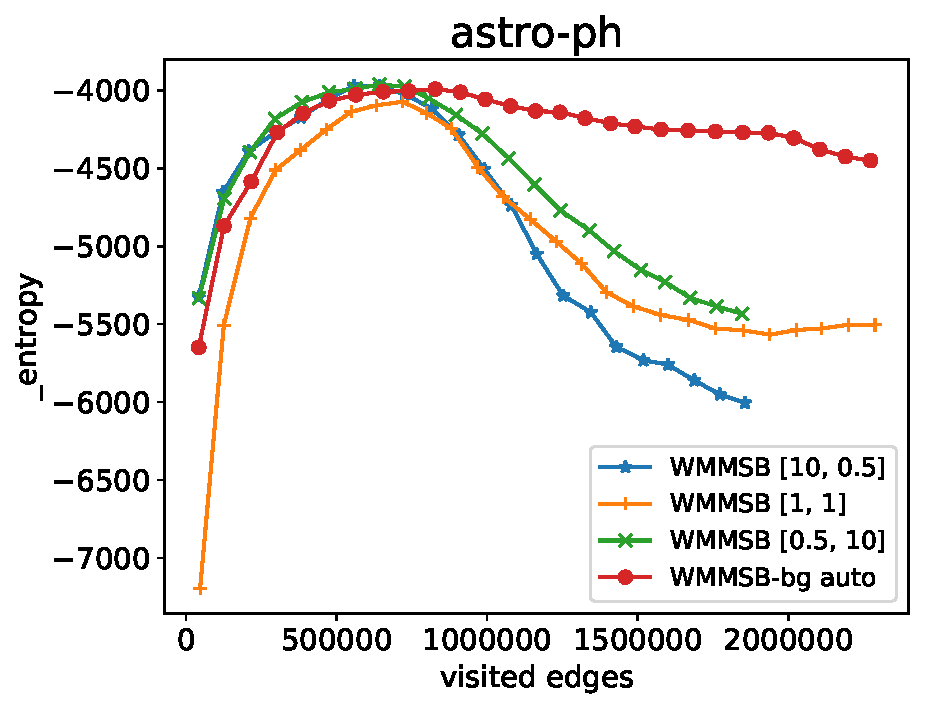
\includegraphics[width=0.32\textwidth]{fig/astro-ph_fig__entropy}
\end{subfigure}
\begin{subfigure}
         \centering
      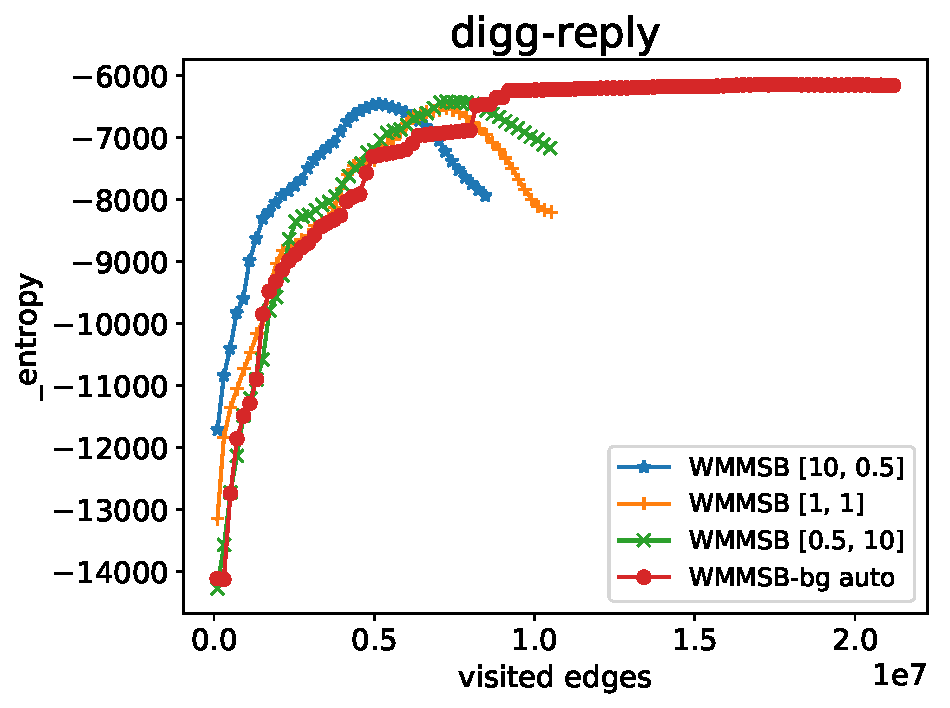
\includegraphics[width=0.32\textwidth]{fig/digg-reply_fig__entropy}               
\end{subfigure}                                                                          
\begin{subfigure}                                                                        
         \centering                                                                      
      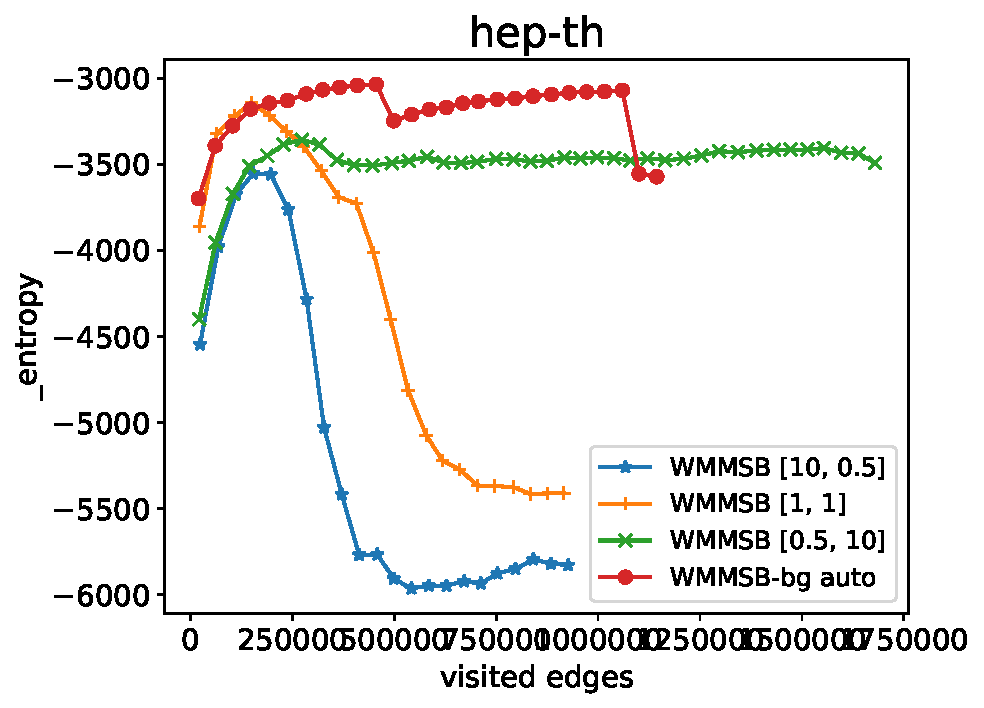
\includegraphics[width=0.32\textwidth]{fig/hep-th_fig__entropy}
\end{subfigure}                                                                          
\begin{subfigure}                                                                        
     \centering                                                                          
         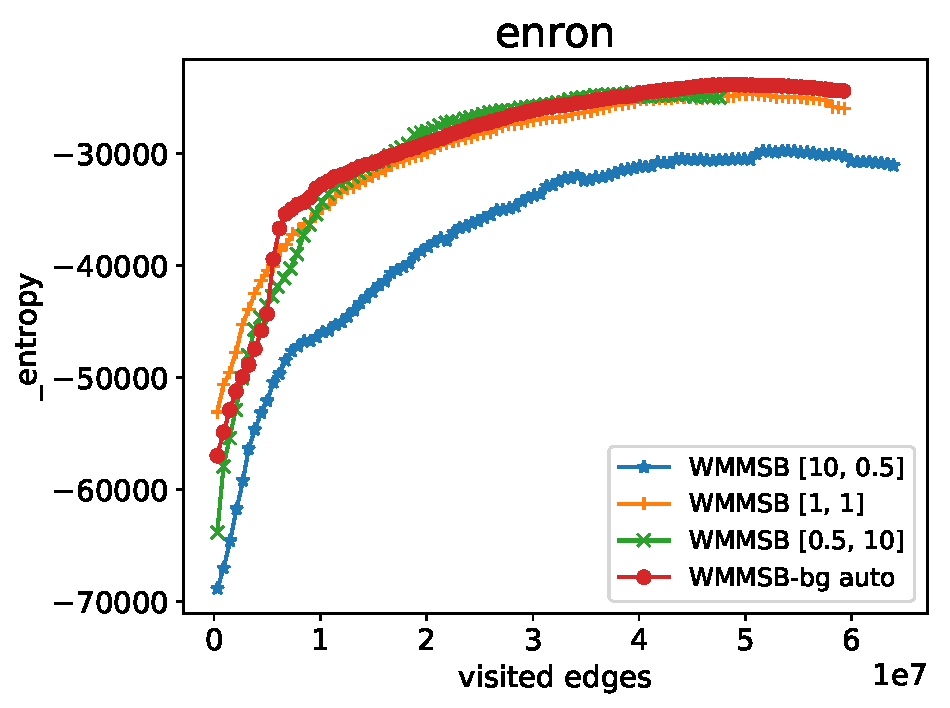
\includegraphics[width=0.32\textwidth]{fig/enron_fig__entropy}
\end{subfigure}
\begin{subfigure}
         \centering
      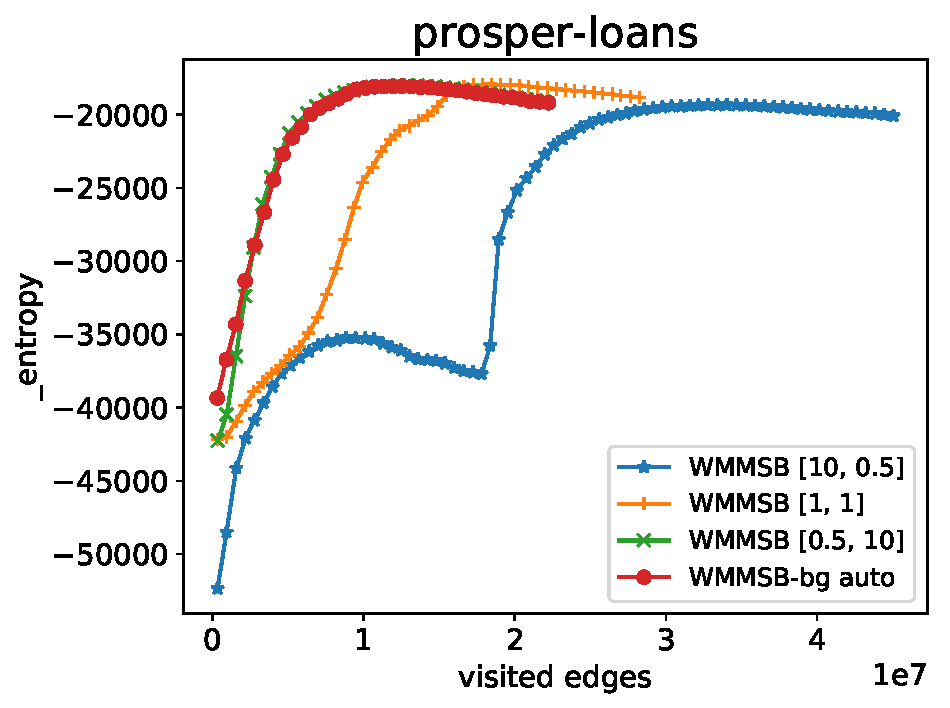
\includegraphics[width=0.32\textwidth]{fig/prosper-loans_fig__entropy}
\end{subfigure}                                                             
\begin{subfigure}                                                           
         \centering                                                         
      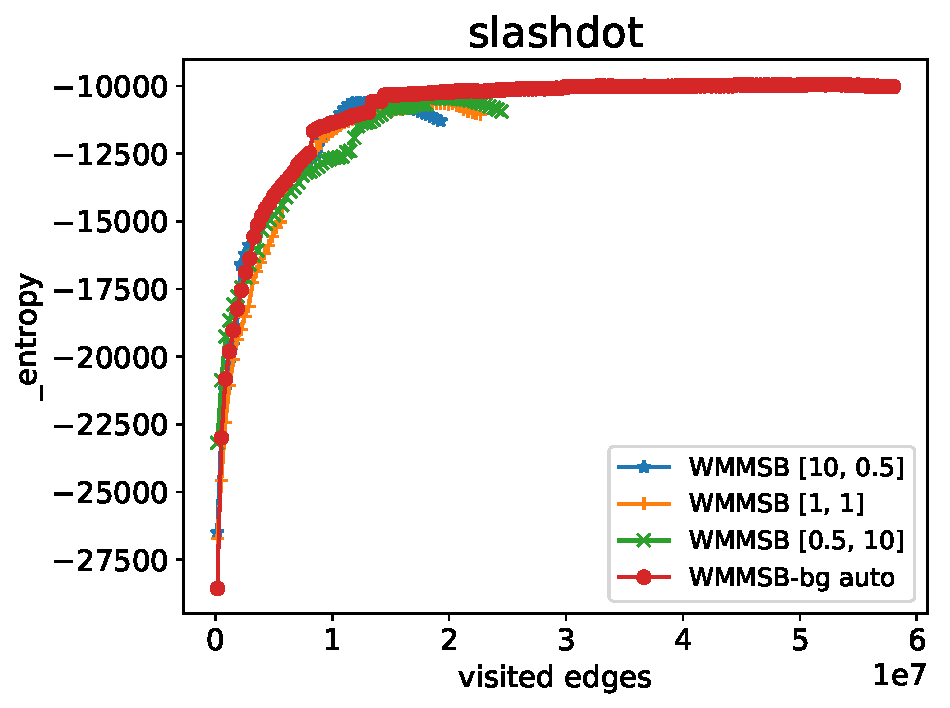
\includegraphics[width=0.32\textwidth]{fig/slashdot_fig__entropy}
\end{subfigure}                                                             
\caption{Log-likehood convergence for WMMSB and WMMSB-bg models. Three different set of hyper-parmeter are used for WMMSB.}


    \label{fig:conv_entropy}
\end{figure}







